\chapter{Background}

\section{vroom}
Vroom is a userspace NVMe driver written in Rust. While it is not production ready at the time of writing, it already provides good performance and the functionality needed for general I/O operations. In comparison to an interrupt driven driver, vroom uses polling to determine the state of the I/O operations. As interrupts are very performance intensive operations, polling can often be better in high-performance environments \cite{spdksubmitting}.
A NVMe driver consists of submission and completion queues, implemented as ring buffers. The driver adds commands to the submission queue, which the NVMe controller reads and executes. The executed command gets placed on a corresponding completion queue.
We unbind the kernel driver and bind it to pci-stub. Pci-stub does not do anything but occupy the pci-driver such that the kernel or another application can not bind to the device.
A sequential vroom I/O operation work as followed:
\begin{itemize}
    \item \textbf{Issue Command:} The application using the driver calls an I/O method on the driver.
    \item \textbf{Pass Command to NVMe:} Vroom creates a struct containing the I/O instructions, placing it onto the head of the submission queue. Vroom then writes to the doorbell register, which notifies the NVMe that a command has to be executed.
    \item \textbf{NVMe I/O:} The NVMe takes the command at the tail of the submission queue. The command is executed through DMA and either writes or reads from the specified LBA on the drive.
    \item \textbf{Completion:} The NVMe controller places the executed submission queue entry on the corresponding completion queue. The waiting driver can then confirm the success of the operation and the application can continue.
\end{itemize}

\section{I/O Memory Management Unit}
Memory Management Units (MMU) for the CPU have been in use since the 1980s. After their first integrated application featuring on Intels 80286 chip \cite{intel80286}, they since have become the defacto standard for addressing memory on computers. By providing processes with a virtual address space instead of physical addresses, every process is isolated and prevented access to memory regions without permission. The MMU uses pages for the translation of addresses. Each address points to a region of memory called a page. These pages can have different sizes, with the default being 4Kib pages on modern x86-64 architectures.

The translation of these pages are stored in a page table structure. A page table structure consists of multiple tables that store parts of the physical address. Certain parts of an address are used as offset in these tables. When an address is translated, a page table walk has to performed. On a 4 level page table structure as the IOMMU uses for 4KiB pages, one address resolution results in 4 memory accesses. Thus, a page table walk is a performance costly operation. To circumvent this, an Translation Lookaside Buffer (TLB) is used to cache translation.

The TLB can store a certain amount of page translations, and is very performant to access. Frequent access to the same address can be done at a fraction of the time needed to perform a page table walk. A TLB miss describes the scenario in which a physical address needs to translated but it has no entry in the TLB, resulting in a expensive page walk.

The advantages and success of the CPUs MMU as well as the introduction of the PCIe bus specification have incentivised Hardware manufacturers to apply this concept on peripheral device busses. In 2006, Intel introduced their "Virtualization Technology for Directed I/O" (VT-d) and AMD their "AMD I/O Virtualization Technology" (AMD-Vi/IOMMU). In this thesis, the term IOMMU references both technologies.

\begin{figure}
    \centering
    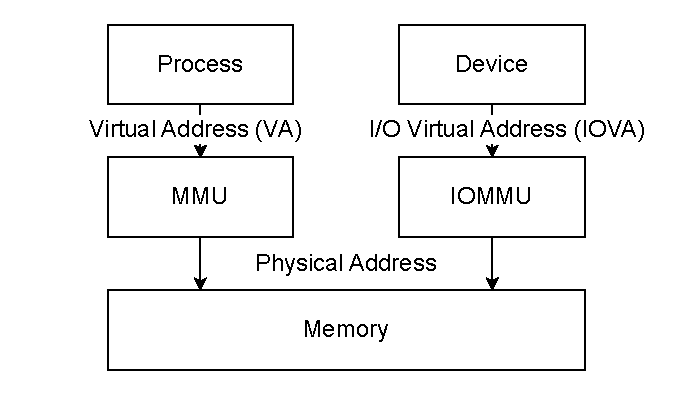
\includegraphics[width=0.5\textwidth]{figures/MMUIOMMU.pdf}
    \caption{MMU and IOMMU relation to memory}
    \label{fig:mmuvsiommu}
\end{figure}

Using DMA Remapping (DMAR) the CPU is bypassed and the direct memory access translated by the IOMMU.
The IOMMU paging structures consist of 4KiB page tables storing 512 8-byte entries. The IOMMU uses the upper portions to determine the location of the stored page tables, and the lower portion of the address as page offset. In the case of \qty{4}{\kibi\byte} pages its 12 bits, for 2MiB its 21.
Mappings can be allocated using the VFIO framework.

\begin{figure}
    \centering
    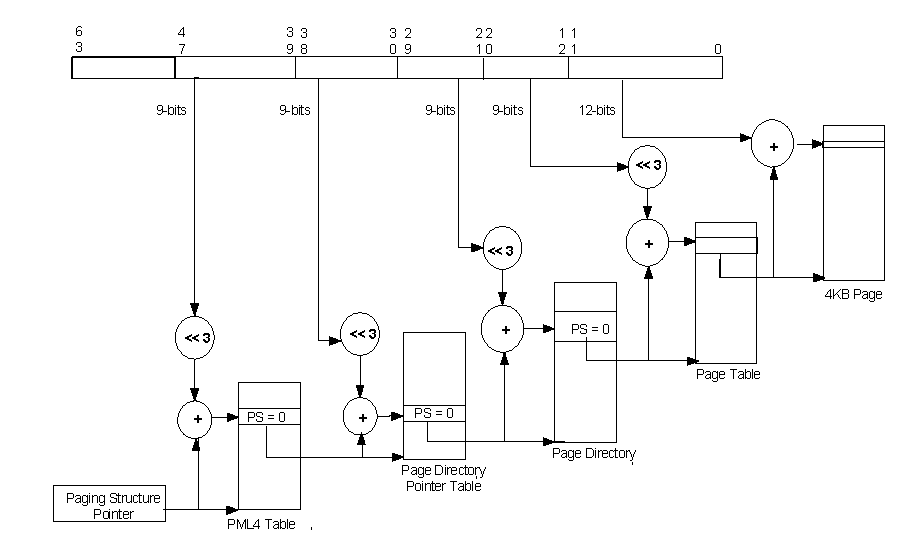
\includegraphics[width=\textwidth]{figures/4kibtranslation.pdf}
    \caption{VT-d Paging structure for translating a 48-bit address to a \qty{4}{\kibi\byte} page}
    \label{fig:pagewalk4kib}
\end{figure}
\begin{figure}
    \centering
    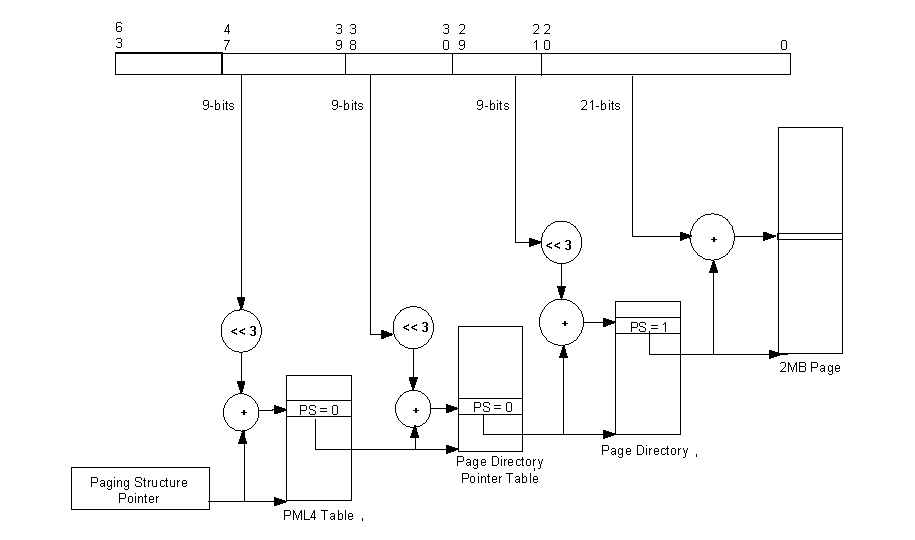
\includegraphics[width=\textwidth]{figures/2mibtranslation.pdf}
    \caption{VT-d Paging structure for translating a 48-bit address to a \qty{2}{\mebi\byte} page}
    \label{fig:pagewalk2mib}
\end{figure}

\section{I/O Translation Lookaside Buffer}
As page table walks are rather costly in performance, a cache on the IOMMU is used to store previously calculated addresses. This cache is called the Input/Output Translation Lookaside Buffer. The IOTLB possesses a limited capacity for entries which is not officially documented.

\section{Memory Mapped I/O}
Memory Mapped I/O, in contrast to Port-Mapped I/O, places Devices in the same address space as the main memory. Instead of using instruction like \texttt{in} or \texttt{out}, a device can be addressed just like the RAM can be. The addressing of this memory itself, can currently be done using two ways. Either accessing it with the physical address, or using a hardware translation device like the I/O Memory Management Unit (IOMMU). Before our implementation, vroom currently only supports the former. % add citation for kernel move/swap

Using the Linux syscall \texttt{mmap(2)} we can create a mapping in the virtual address space of our process. These mapping use so-called Pages. Pages are units of memory with a predefined size, the pagesize. The supported pagesizes can differ depending on the cpu architecture. As we use x86-64 for our tests, we have the default pagesize of \qty{4}{\kibi\byte} and the bigger pagesizes \qty{2}{\mebi\byte} and \qty{1}{\gibi\byte}. Pages allocated with these bigger pagesizes are called Hugepages. In addition to mapping memory into our virtual address space, calling \texttt{mmap} with no address can be used as an allocation method for big data amounts \cite{mmapmanpage}.

\section{Direct Memory Access}
Using Direct Memory Access we can bypass the CPU for I/O operations. Previously this was handled by a separate DMA-controller hardware (third-party DMA) but using PCI, we can directly access it through bus mastering (first-party DMA). Using the IOMMU the request gets intercepted and translated to the physical address.

\section{Hugepages}
As the demand for bigger memory mappings e.g. for big files increased, the amount of TLB cache misses rose proportionally. With the CPUs TLB having space for only 4096 \qty{4}{\kibi\byte} pages, only an address space of 16MiB could be stored and accessed quickly. In order to increase the amount of virtual memory space, hardware producers reacted by providing bigger page sizes on their architectures than the default \qty{4}{\kibi\byte}.
Linux currently provides two ways of using Hugepages.
In the optimal case, using a \qty{2}{\mebi\byte} or \qty{1}{\gibi\byte} page size should result in a 512 or 262144 times reduction in cache misses compared to \qty{4}{\kibi\byte} pages. Especially in high-performance computing this make a huge difference.

\begin{itemize}
    \item \textbf{Persistent Hugepages}: Persistent Hugepages, are reserved in the kernel and cannot be swapped out or used for another purpose. To use these hugepages, they are mounted as a (pseudo) filesystem called hugetlbfs, which lays in the directory \texttt{/mnt/huge}. The amount and size of the pages can be specified either during boot on the kernel commandline with e.g. \texttt{hugepagesz=1g hugepages=16} or dynamically using the Linux \texttt{sysfs} pseudofilesystem e.g. \texttt{echo 16 > /proc/sys/vm/nr\_hugepages}\cite{hugetlbkerneldocs}.
    \item \textbf{Transparent Hugepages}: Transparent Hugepages are a more recent addition to the kernel. Transparent hugepages are not fixed or reserved in the kernel and allow all unused memory to be used for other purposes. THPs provides a way of utilising the TLB effectively without reserving huge amounts of memory. The \texttt{khugepaged} daemon scans memory and collapses sequences of basic pages into bigger pages. THPs can either be enabled, disabled or only be used on \texttt{madvise(MADV\_HUGEPAGE)} memory regions \cite{transhugekerneldocs}.
\end{itemize}

vroom currently uses hugepages and locks them using mlock to prevent the Kernel from swapping them out. In order to 'pin' pages, preventing the Linux Kernel from switching them around, Hugepages have to be used. The kernel does not have the ability to move these pages like 4KiB pages.
For accessing the devices memory as well as the device accessing the host memory, it is necessary to either use the physical addresses and compromise on safety and use root privileges or use the IOMMU for virtualization, which can introduce performance overhead.

\section{Peripheral Component Interconnect Express}
\paragraph{Address Translation Service}


\subsection{Character and Block Devices}
Unix/Linux use two types of devices: Character and Block devices. Character devices are used for devices with small amounts of data and no frequent seek queries, like keyboard and mouse. Block devices on the other hand have a large data volumes, which are organized in blocks and where search is common, like harddrives and ram disks.
Read and Write operations on character devices are done sequentially byte-by-byte, while on block devices, read/write is done at the data block level.
These constraints also impact how the drivers for these devices work. CDev drivers directly communicate with the device drivers, while block device drivers work in conjunction with the kernel file management and block device subsystem. This allows efficient asynchronous read/write operations for large data amounts, but small byte sized data transfer achieves lower latency on character devices.

\subsection{Rust}
While userspace drivers can theoretically and practically be written in any language, as proven by the network driver Ixy \autoref{s:ixy}, Rust excels as it not only offers memory-safety but memory-safety without garbage collection. This is especially important, as garbage collected languages have overhead and latency spikes, which can lower performance. Another huge factor is that Rust, like C, does not use exceptions. By handling, or even better, being forced to handle errors assures that no rogue exception can take down critical code infrastructure.
Additionally, Rust provides low-level access while also offering a high-level development experience through zero-cost abstractions.